% 2011 年广东卷理科第 18 题：锥体 P-ABCD，ABCD 是边长为 1 的菱形，∠DAB=60°，
%   PA=PD=√2，PB=2，E、F 分别是 BC、PC 的中点。
% 来源 PDF：普通高考/2011/2011广东理.pdf，SHA-256 676f6eb7aaa62d199da64d67e0951301d980eb1e4d82193579afc4a4637ac874。
% 原页：第 1 页（A3 三栏）第 3 栏下部，书页码 663。
% 重绘依据（源为矢量，坐标取自 pdftocairo SVG，真页 pt、原点左上、y 向下）：
%   P(976.3,522.2)、A(1019.9,620.6)、B(1099.3,620.6)、C(1133.0,600.7)、D(1053.7,600.7)、
%   E(1116.1,610.7)、F(1054.7,561.5)；其中 E 为 BC 中点、F 为 PC 中点（与原页坐标吻合）。
%   实线：PA、PB、PC、AB、BC、EF；虚线（被遮挡）：PD、DA、DC、DE、DF。照源不改。
%   本图取本地坐标 (x,y)=(x_page−960, 660−y_page)，1 单位 = 1 TeX pt，y 向上；
%   拓扑与原页一致，不按原页绝对比例。
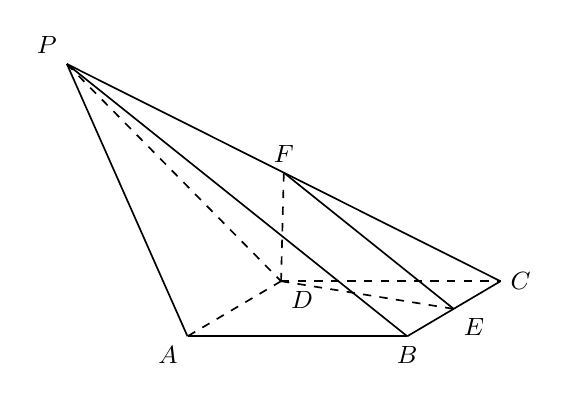
\begin{tikzpicture}[x=1pt, y=1pt, >=stealth, semithick, font=\small]
  \coordinate (P) at (16.3,137.8);
  \coordinate (A) at (59.9,39.4);
  \coordinate (B) at (139.3,39.4);
  \coordinate (C) at (173.0,59.3);
  \coordinate (D) at (93.7,59.3);
  \coordinate (E) at (156.1,49.3);
  \coordinate (F) at (94.7,98.5);
  % 被遮挡的棱与辅助线（原页为虚线）
  \draw[dashed] (P) -- (D);
  \draw[dashed] (D) -- (A);
  \draw[dashed] (D) -- (C);
  \draw[dashed] (D) -- (E);
  \draw[dashed] (D) -- (F);
  % 可见的棱与辅助线（原页为实线）
  \draw (P) -- (A);
  \draw (P) -- (B);
  \draw (P) -- (C);
  \draw (A) -- (B);
  \draw (B) -- (C);
  \draw (E) -- (F);
  % 顶点标注（位置照原页）
  \node[above left] at (P) {$P$};
  \node[below left] at (A) {$A$};
  \node[below] at (B) {$B$};
  \node[right] at (C) {$C$};
  \node[below right] at (D) {$D$};
  \node[below right] at (E) {$E$};
  \node[above] at (F) {$F$};
\end{tikzpicture}
